

\chapter{Étude de la structure d'un flot de liens réel}

L'étude\note{Intro surement trop général qui sera bougée ailleurs.}\ de la structure des réseaux est un sujet qui est étudié depuis assez longtemps \REF.
Ces études ont, dans un premier temps, permis de trouver comment caractériser une structure puis, dans un second temps, de proposer des méthodes de détections de ces structures.
La littérature sur l'étude des flots de liens est encore récente et il n'existe que peu d'études \REF\ sur les spécificités des structures dans les flots de liens.

Nous nous intéressons ici à une archive de courriels publiquement disponibles\footnote{\url{https://lists.debian.org/debian-user/}}.
Cette archive contient l'ensemble des courriels échangés par différent utilisateurs pour résoudre un problème survenu lors de l'utilisation de Debian.
Typiquement, une personne ayant un problème lors de l'installation envoie un courriel à la liste afin de demander de l'aide.
Toutes personnes inscrites sur la liste reçoit ce courriel et peut y répondre ce qui donne lieu à une discussion visible par tous.
Ces discussions ont déjà été étudiées dans le passé~\cite{Dorat2007} mais cela a été fait en utilisant des méthodes statique uniquement.

Hors, ces données se transposent facilement sous forme de flot de liens en transformant une personne en un n\oe uds et chaque courriel entre deux personnes en un lien dans le flot à l'instant où le courriel a été envoyé.
L'avantage de ces données de communications est que nous connaissons la discussion dans laquelle a lieu chaque message.
Une discussion est un ensemble de courriels dont tout les messages répondent à un message précédant de la discussion excepté pour le premier qui a initié la discussion et que nous appelons \emph{racine}.
Ainsi, nous étudions la structure des discussions dans le flot liens représentant les courriels envoyés sur la liste.

Utiliser le formalisme de flot de liens est particulièrement intéressant car cette lite de diffusion existe depuis 1994.
L'aspect temporelle des discussions est donc important.



\section{Prétraitement sur le jeu de données}
Bien que accessible sur internet, ce jeu de données nécessite un ensemble de traitement avant de pouvoir exploiter les 724985 courriels que contenait l'archive en janvier 2015.
Tout d'abords, les données ne sont pas sous la forme d'un flot de liens avec la structure des conversations.
Les données sont accessibles via le site internet et ne sont pas structurées.
Pour avoir ces informations sous la forme d'un flots de liens, un script d'extraction a été développé \com{URL}.
Lors de l'extraction, 2269 courriels n'ont pas pu être pris en compte car certaines informations étaient manquantes ou mal formées.

Une fois les informations récupérées, il faut les transformer en un flot de liens.
Pour chaque message $m$, nous extrayons son auteur $a(m)$, l'instant $t(m)$ auquel le message a été posté\,\footnote{Cet instant est convertit en $timestamp$ en tenant compte des fuseaux horaires.}, le message auquel il réponds $p(m)$ trouvé via le champ \textsc{In-Reply-To}, son destinataire $a(p(m))$ et la discussion $D(m)$ dans laquelle il apparait.
Comme les messages \emph{racines} ne répondent à aucun autre, nous imposons $p(m)=a(m)$.
L'ensemble de liens du flot est donc $\{t(m),a(m),a(p(m))\}_m$.

Une fois le flot créé, il est encore nécessaire de vérifier sa cohérence.
Un message peut être filtré pour différentes raisons: le courriel apparait avant le message auquel il est censé répondre, le message auquel il réponds n'est pas présent dans l'archive, l'auteur et le destinataire sont la même personne\footnote{Cela concerne principalement les \emph{racines}}.
Cette dernière condition permet notamment d'éviter la présence de boucle dans le flot.
Il s'agit de vérifications simple auquel il faut ajouter les vérification de la cohérence de la structure des discussions.
Ainsi, une discussion est entièrement retirée du jeu de données si il manque la \emph{racine},si un de ces messages a été retiré à l'étape précédante ou si la discussion a débuté trop récemment ou si elle dure trop longtemps.
Les deux dernières conditions permettent d'éviter un biais envers les conversations incomplètes car trop longues ou trop récentes.
La limite pour considérer une discussion trop récente ou trop longue a été fixé à 2 ans en observant la distribution de durées des discussions, voir la figure~\ref{fig:dists_discussion}.

Une fois tout ces messages filtrés, nous obtenons un flot de liens avec 554233 liens entre 34648 personnes pendant presque 19 ans et 116999 discussions.
Mis à part les messages de début de discussions, se sont 53753 courriels qui ont été filtrés soit environ $7\%$.
\inline{+ parler que les mails sont sans durée et que l'on ajoute delta par la suite?}
\section{Caractéristiques basiques des discussions}

Les caractéristiques les plus basiques des discussions sont les nombres de courriels, les nombres de personnes, les nombres de paires de personnes distincte en interaction direct et leurs durées.
Sur la figure~\ref{fig:dists_discussion}, sont présentées les distributions cumulatives inverses de ces notions et on remarque qu'elles sont toutes hétérogènes.
On remarque que les données filtrées ne diffèrent pas qualitativement des données brutes

\begin{figure}
\centering
	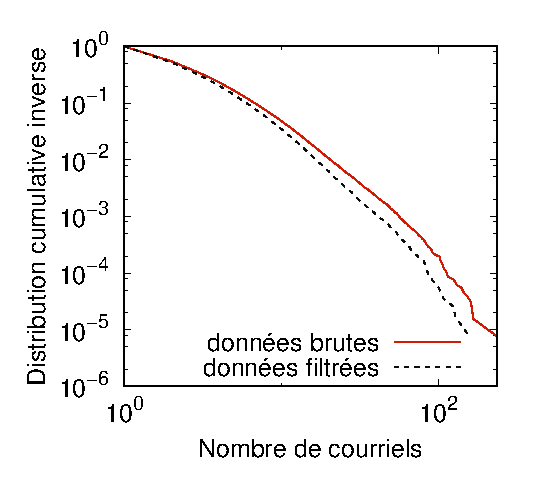
\includegraphics[angle=-90, width=0.49\linewidth]{img/mailing/sizes-ccdf.eps}
	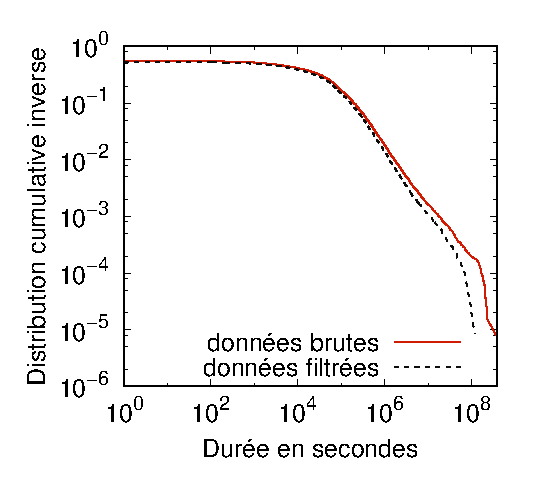
\includegraphics[angle=-90, width=0.49\linewidth]{img/mailing/durations-ccdf.eps}\\
	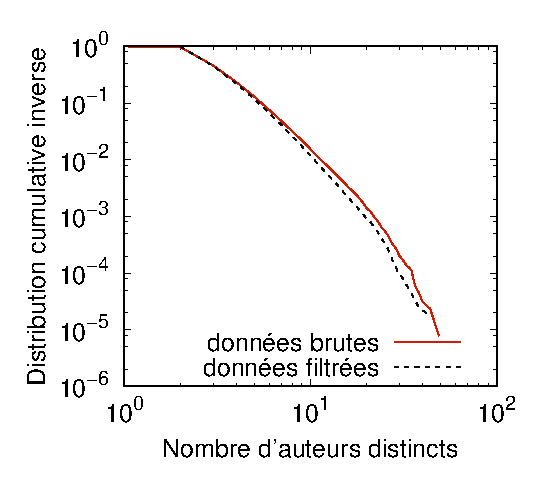
\includegraphics[angle=-90, width=0.49\linewidth]{img/mailing/authors-ccdf.eps}
	\includegraphics[angle=-90, width=0.49\linewidth]{img/mailing/authorpairs-ccdf.eps}
	
	\caption{Distribution cumulative inverse de différentes caractéristiques pour les données brutes (ligne pleine) et filtrées (ligne pointillé). En haut à gauche: nombre de courriels dans une discussion; en haut à droite: durée d'une discussion; en bas à gauche: nombre de personnes dans une discussion; en bas à droite: nombre de paires d'auteurs distinct dans une .}
	\label{fig:dists_discussion}
\end{figure}

La distribution des durées des discussions montre que la majorité des discussions dure environ une journée ou moins (100000 secondes équivaux à moins de 28 heures).
Par ailleurs, on remarque qu'il n'existe que quelques discussions durant plus d'un an.
C'est pourquoi, la limite sur la durée des discussions a été fixée à 2 ans.

Ces premières observations sont nécessaires mais pas suffisante pour comprendre les caractéristiques d'une discussion.
Nous avons également étudié la corrélation de ces différentes notions et une partie d'entre elles sont présentées sur la figure~\ref{fig:corr_discussion}.


\begin{figure}
	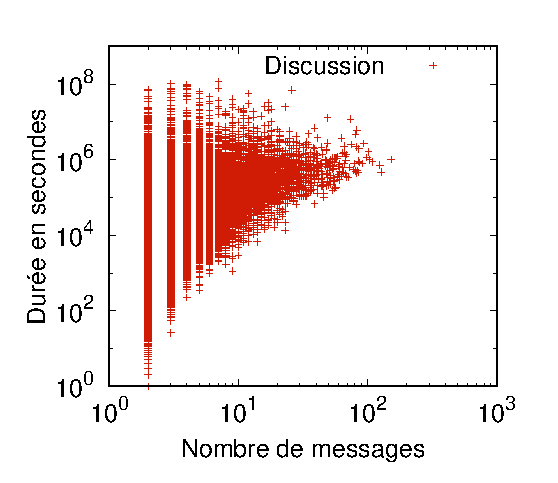
\includegraphics[angle=-90, width=0.49\linewidth]{img/mailing/sizes-durations-corr.eps}
	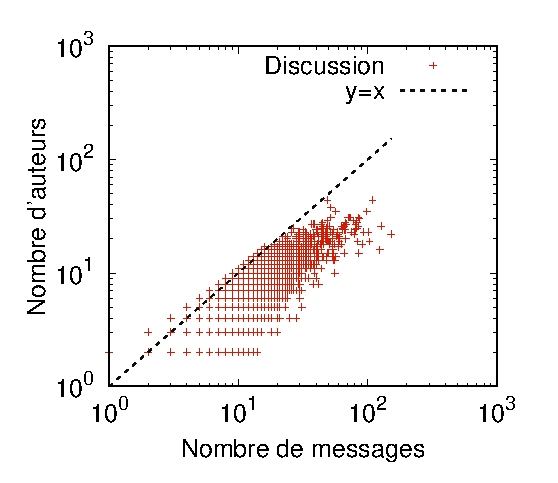
\includegraphics[angle=-90, width=0.49\linewidth]{img/mailing/sizes-authors-corr.eps}
	\caption{Gauche: Corrélations entre le nombre de courriels et la durée d'une discussion. Droite: Corrélation entre le nombre de courriels et le nombre d'auteurs dans une discussion.}
	\label{fig:corr_discussion}
\end{figure}

La corrélation entre la durée et le nombre de courriels, sur la figure~\ref{fig:corr_discussion} partie gauche, mets en évidence que plus une discussion est grande en nombre de courriels plus elle dure longtemps ce qui est attendu.
Par contre, on observe que les petites discussions ont des durées très variables. 
Sur la partie droite de la figure~\ref{fig:corr_discussion} présentant la corrélation entre le nombre de courriels et d'auteurs, on observe un autre fait attendu~\cite{Dorat2007} qui est qu'une discussion est constitué de plus de messages que de participants.
Ainsi lors d'une discussion, c'est un petit nombre de personnes qui partagent potentiellement beaucoup de messages. 

Enfin, il est intéressant d'observer la dynamique des échanges entre deux personnes.
Soit $\tau(u,v) = (t_{i+1}-t_i)_{i=0..k+1}$ la séquence des temps inter-contacts de $k$ liens entre les n\oe uds $u$ et $v$ où $t_0$ est le temps entre $\alpha$ et le premier lien et $t_{k+1}$ est le temps entre le dernier lien et $\omega$.
Il s'agit du temps écoulé avant que deux personnes se contactent à nouveau.
Sur la figure~\ref{fig:ict_discussion} est représentée la distribution cumulative inverse du temps inter-contacts. 
On remarque que $21\%$ des temps inter-contacts est inférieurs à 30 jours.
Ce chiffre bien que relativement faible est tout de même important car il s'agit de discussions ouvertes où tout le monde peut participer. 
En particuliers, une personne peut envoyer une demande d'aide à un moment donner et ne plus jamais échanger avec les même personnes.
Or, on observe que 21\% des contacts sont renouvelés en moins de 30 jours.
La participation est donc quand relativement élevée.
\begin{figure}
	\centering
	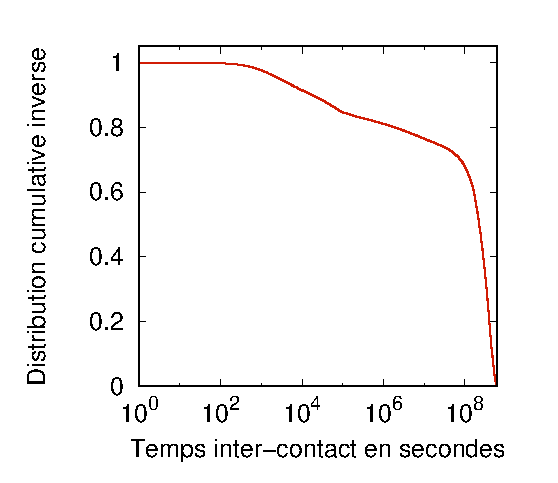
\includegraphics[width=0.49\linewidth]{img/mailing/ict-ccdf.eps}
	\caption{Distribution des temps inter-contacts dans le fil de discussions.}
	\label{fig:ict_discussion}
\end{figure}

\section{\'Etude des discussions en tant que sous-flots}
\subsection{Application de la $\Delta$-densité}
\label{delta_densite}

Jusqu'à maintenant aucune notion intrinsèquement liée aux flots de liens n'a été utilisée pour caractériser les discussions.
Le but est d'évaluer si cette structure de flot peut se rapprocher d'une structure communautaire.
Comme dit précédemment, les communautés sont souvent définies comme étant des structures devant être densément connectées.
C'est pourquoi nous nous attachons à étudier la densité des discussions.

Comme ces données se modélisent par un flot de liens ou chaque lien n'a pas de durée, nous étudions la $\Delta$-densité pour différentes valeurs de $\Delta$ entre 1 seconde et 20 ans.
Tout d'abord sur la figure~\ref{fig:dens_fil_discusion} est représenté la $\Delta$-densité globale du le flot.
En couvrant un spectre aussi large de $\Delta$, on observe que la $\Delta$-densité est croissante avec $\Delta$ mais surtout on observe bien la convergence de $\Delta$-densité vers $3.139\times 10^{-4}$, la densité du graphe agrégé, lorsque $\Delta$ est proche de $\omega - \alpha$.

\begin{figure}
	\centering
	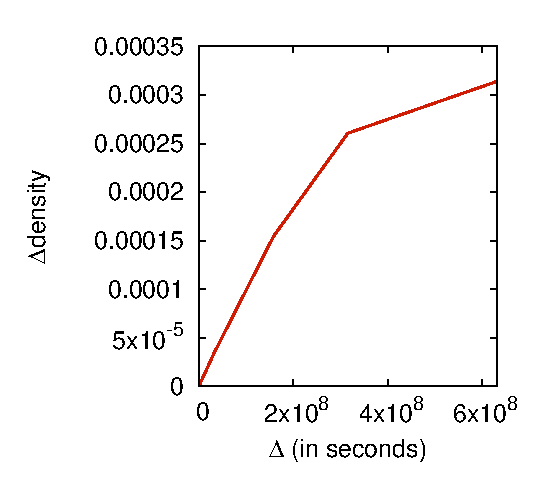
\includegraphics[width=0.48\linewidth]{img/mailing/global_linlin.eps}
	\caption{Évolution de la $\Delta$-densité du flot de liens pour $\Delta$ de $1$ seconde à $20$ ans. \com{Ajout bar horizontal de la densité statique dans le graphe agrégé.}}
	\label{fig:dens_fil_discusion}
\end{figure}

Cependant, la $\Delta$-densité du flot n'apporte que peu d'informations en elle-même.
Elle est surtout utile pour comparer les valeurs de $\Delta$-densité des sous-flots que sont les discussions.
Ainsi sur la figure~\ref{fig:intra_dens_discussion}, est présentée la distribution cumulative inverse de la $\Delta$-densité des discussions pour différentes valeurs de $\Delta$.
On remarque que les différentes valeurs de $\Delta$ ne semblent pas influencer qualitativement la distribution de $\Delta$-densité.
Cette courbe mets surtout en évidence que les discussions sont des structures beaucoup plus denses que le flot.
En effet, la densité médiane des discussions est, selon la valeur de $\Delta$, entre $2.69 \times 10^{-4}$ et $0.28$ alors que le flot a une $\Delta$-densité variant entre $1.05  \times 10^{-10}$ et $3.42 \times 10^{-5}$.
La $\Delta$-densité des discussions est donc en moyenne $10^{5}$ fois plus élevé que celle du flot.
Bien que notable, ce fait est attendu notamment car le flot dure beaucoup plus longtemps et concerne beaucoup plus de n\oe uds que les discussions.
\begin{figure}
\centering
%\subfloat[Inverse cumulative distribution of intra-threads density.]{
	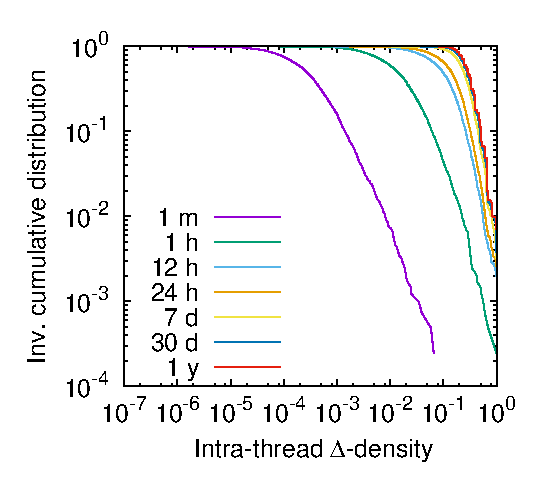
\includegraphics[width=0.48\linewidth]{img/mailing/delta.eps}
%}

\caption{Distribution cumulative inverse de la $\Delta$-densité des discussions pour différentes valeurs de $\Delta$s.}
\label{fig:intra_dens_discussion}
\end{figure}

Afin d'aller plus loin dans l'étude de cette structure, il faut revenir à une définition plus précise de ce qu'est une bonne communauté.
En soit, une valeur de densité n'est pas suffisante pour définir une structure communautaire.
En effet, une discussion ayant une densité de $0.8$ peut  ne pas être une communauté tant dis qu'une autre ayant une densité proche de zéro peut être une communauté.
Il faut définir un point de comparaison pour effectivement affirmer qu'une structure est particulièrement dense.
La prise en compte de la densité globale est un début mais n'est pas suffisante.

Une autre définition d'une communauté est qu'elle devrait être plus densément connecté à l'intérieur qu'avec les autres communautés adjacentes.
Pour un graphe $G=(V,E)$ et une communauté $C_i$ de la partition $C = \{C_j\}_{j_1..k}$ de $V$ en $k$ communautés, cela se traduit par le calcul de la densité entre les communautés, $\delta^{inter}(C_i)$ :

\begin{equation}
	\delta^{inter}(C_i) = \frac{1}{|C|-1}\sum_{j, i\ne j}\frac{|\{(u,v)\in E\mbox{ t.q. }u\in C_i\mbox{ and }v\in C_j\}|}{|C_i|\cdot |C_j|}.
\end{equation}
Il s'agit tout simplement de la probabilité qu'un lien existe entre les n\oe uds des deux communautés.
Encore une fois, cette notion n'a pas de sens direct dans le formalisme de flot de liens et il est nécessaire de l'adapter.
Pour ce faire, nous définissons la $\Delta$-densité inter discussions entre deux discussions $D_i$ et $D_j$: $\delta^{inter}_{\Delta}(D_i,D_j)$.
Soit $L'= \xi(L,\Delta)$, $V'= V(D_i) \cup V(D_j)$, $t_{\beta}'=t_{\beta}(D_i \cup D_j)$ et $t_{\psi}'=t_{\psi}(D_i \cup D_j)$.
La définition de $\delta^{inter}_{\Delta}(D_i,D_j)$ est la suivante: $\delta^{inter}_{\Delta}(D_i,D_j) = d(L_{t_{\beta}'..t_{\psi}'}'(V'))$.
Il s'agit donc de la $\Delta$-densité du flot de liens induit par l'union des n\oe uds sur l'union de l'intervalle\note{Faire un dessin de cette situation?}.
Afin d'obtenir la $\Delta$-densité inter discussions entre $D_i$ et tout les autres discussions, nous utilisons la moyenne des densité inter discussion entre $D_i$ et les autres discussions, soit:

\begin{equation}
	\delta^{inter}_{\Delta}(D_i) = \frac{1}{|C|-1}\sum_{j,i\ne j} \delta^{inter}_{\Delta}(D_i,D_j).
\end{equation}

La distribution cumulative inverse de la $\Delta$-densité inter discussions est sur la figure~\ref{fig:inter_dens_discussion} pour différentes valeurs de $\Delta$.
Bien que similaire, le comportement de la $\Delta$-densité inter discussions diffère qualitativement de celui de la $\Delta$-densité.
La $\Delta$-densité inter discussions croit également en fonction de $\Delta$ mais il y a toujours une différence notable entre $\Delta= 1\  mois$ et $\Delta= 1\ an$ ce qui n'est pas le cas pour la $\Delta$-densité.
Cette différence est normale car lors du calcul de $\Delta$-densité le nombre de liens considérés est fixe peut import $\Delta$ alors qu'il croit avec $\Delta$ lors du calcul de $\Delta$-densité inter discussions.
Un autre facteur est aussi la duré considérée, $t_{\psi}'-t_{\beta}'$, qui est plus longue que la durée des discussions.
\begin{figure}
\centering
%\subfloat[Inverse cumulative distribution of inter-threads density.]{
	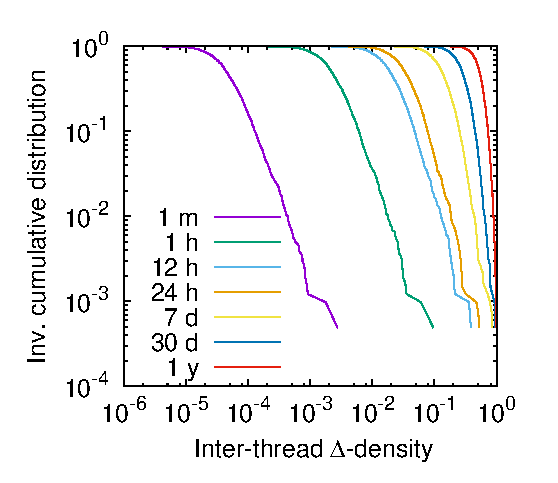
\includegraphics[width=0.48\linewidth]{img/mailing/inter_delta.eps}
%}
\caption{Distribution cumulative inverse de la $\Delta$-densité inter discussions pour différentes valeurs de $\Delta$s.}
\label{fig:inter_dens_discussion}
\end{figure}


Afin de comparer plus aisément $\Delta$-densité et $\Delta$-densité inter discussions, la corrélation entre ces deux mesures est présentée sur la figure~\ref{fig:corel_inter_discussion} pour différentes valeurs de $\Delta$.
On remarque que les discussions sont effectivement plus denses intérieurement qu'avec les autres discussions.
La différence est de plusieurs ordres de grandeur lorsque $\Delta$ est petit et elle diminue lorsque $\Delta$ croit.
Pour $\Delta=20\ ans$ sur la figure~\ref{fig:corel_inter_discussion_20}, la différence n'est plus visible car à cette échelle de temps, l'ancrage temporel des discussions n'est plus décisif.
On remarque tout de même que pour $\Delta=1\ an$, la différence reste notable.
 

\begin{figure}[]
\centering
\subfloat[$\Delta= $1 minute]{
	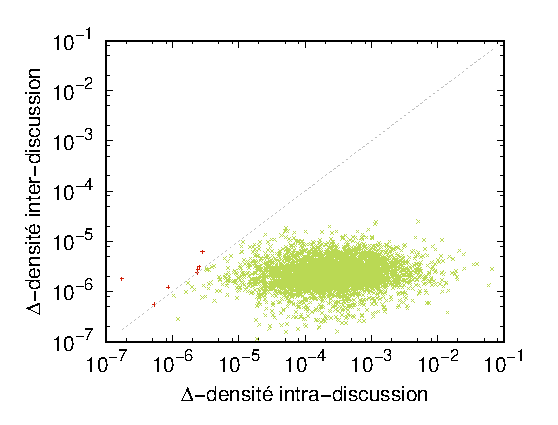
\includegraphics[width=0.48\linewidth]{img/mailing/DensityCurve/120/mean.eps}
}
\subfloat[$\Delta= $1 jour]{
	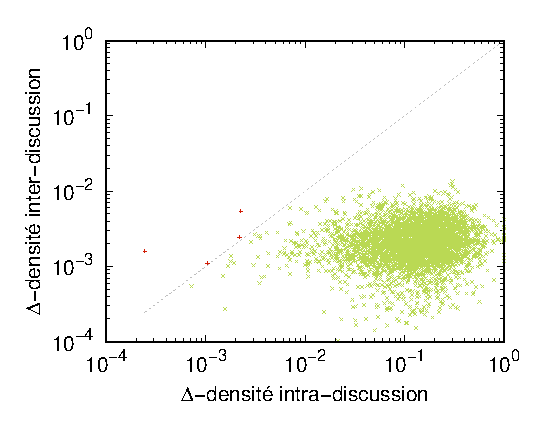
\includegraphics[width=0.48\linewidth]{img/mailing/DensityCurve/172800/mean.eps}
}

\subfloat[$\Delta= $1 an]{
	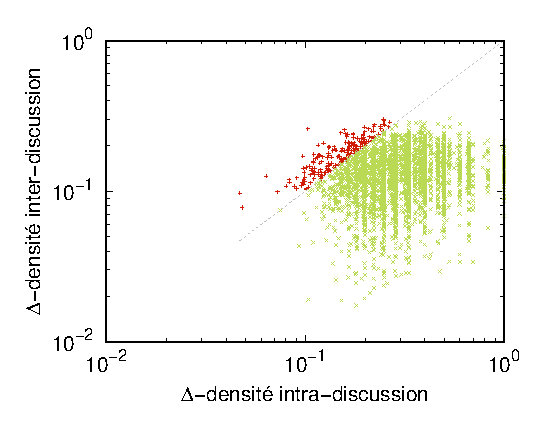
\includegraphics[width=0.48\linewidth]{img/mailing/DensityCurve/63072000/mean.eps}
}
\subfloat[$\Delta= $20 ans]{\label{fig:corel_inter_discussion_20}
	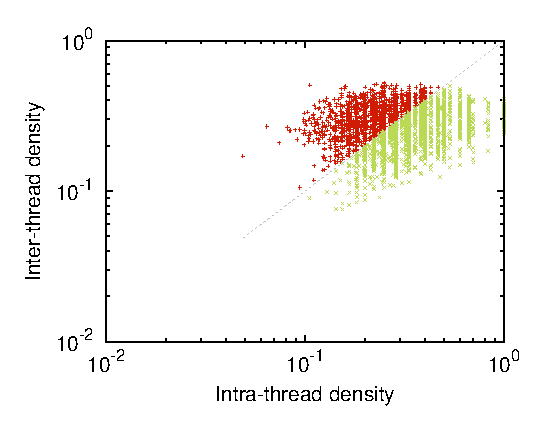
\includegraphics[width=0.48\linewidth]{img/mailing/DensityCurve/1261440000/mean.eps}
}
\caption{Corrélations entre $\Delta$-densité et $\Delta$-densité inter discussions pour différentes valeurs de $\Delta$. Une discussion est en vert (resp. rouge) si elle a une $\Delta$-densité plus (resp. moins) élevée que sa $\Delta$-densité inter discussions.}
\label{fig:corel_inter_discussion}
\end{figure}

\subsection{Répartition temporelle et structurelle des discussions}

Nous avons étudié la densité des discussions et entre les discussions mais il est également intéressant d'observer comment ces discussions sont réparties topologiquement et temporellement.
Pour étudier la répartition des discussions dans le temps, nous construisons un graphe d'intervalle \REF $X=(V_X,E_X)$ représentant le chevauchement temporel.
Chaque discussion du flot devient un n\oe ud de $V_X$ et le lien $(i,j)$ existe dans $E_X$ si les discussions $D_i$ et $D_j$ correspondantes ont eu lieu au même instant, \emph{i.e.} $[\alpha_i, \omega_i] \cap [\alpha_j, \omega_j] \neq \emptyset$.
De manière similaire, nous définissons le graphe de chevauchement topologique $Y=(V_Y,E_Y)$.
Les n\oe uds de se graphe représentent encore une fois les discussions du flot et un lien existe entre deux discussions si au moins une personne a participé aux deux, \emph{i.e.} $V(D_i) \cap V(D_j) \neq \emptyset$.

Ces deux graphes sont constitués de 116999 n\oe uds et de environ 2 millions de liens pour le graphe de chevauchement temporel et de environ 63 millions de liens pour le graphe de chevauchement topologique.
Par construction, ces graphes contiennent beaucoup d'informations sur les relations entre les discussions.


Sur la figure~\ref{fig:x-y-graphs_discu}(gauche), est représentée la corrélation entre le degré d'une discussion dans le graphe de chevauchement temporel $X$ et sa durée.
Il y a une corrélation évidente entre ces deux notions lorsque les discussions ont une durée supérieur à $10^5$ secondes.
Plus une discussion dure longtemps, plus elle a de chance d'avoir lieu en même temps que beaucoup d'autres discussions.
On observe également que, même pour les discussions durant moins d'un jours ($8.6 \times 10^4$\,s), il y a jusqu'à une centaine d'autres discussions actives sur la même période.

\begin{figure}
\centering
	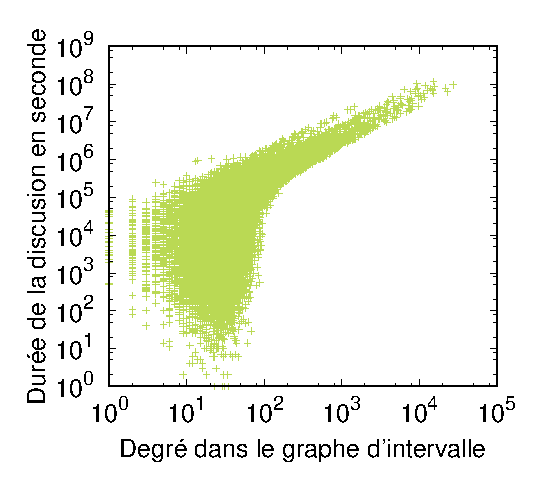
\includegraphics[width=0.49\linewidth]{img/mailing/degree_temp}
	\hfill
	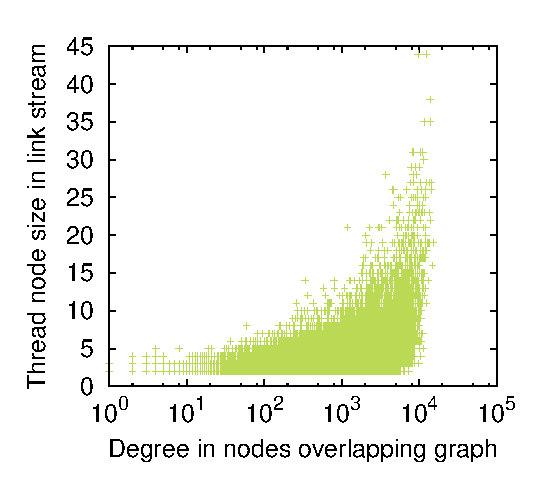
\includegraphics[width=0.49\linewidth]{img/mailing/degree_nodes}
	\caption{Gauche: Corrélation entre le degré des discussions dans le graphe de chevauchement temporel et leur durée. Droite: Corrélation entre le degré des discussions dans le graphe de chevauchement topologique et leur nombre de participants.}
	\label{fig:x-y-graphs_discu}
\end{figure}

La figure~\ref{fig:x-y-graphs_discu}(droite) présente la corrélation entre le degré d'une discussion dans le graphe de chevauchement topologique $Y$ et son nombre de participants.
La corrélation est moins nette mais il y a tout de même une tendance.
Par contre, on remarque de manière frappante que même une petite discussions partagent énormément de n\oe uds avec les autres discussions.


\subsection{Flot quotient}

Le graphe quotient\REF\ est une autre notion clef pour étudier les relations entre les communautés d'un graphe $G=(V,E)$.
Soit une partition $C= \{C_i\}_{1 .. k}$ des n\oe uds de $G$ en $k$ communautés, chaque communauté est représentée dans le graphe quotient $\bar{G}$ par un n\oe uds dans $V$.
Il y a un lien entre deux communauté $C_i$ et $C_j$ dans $E$ si il existe au moins un lien entre un n\oe uds de $C_i$ et un n\oe uds de $C_j$.
Voir une illustration sur la figure~\ref{fig:graph-quotient}.
Il est possible d'ajouter un poids sur les liens de $\bar{G}$ égale au nombre de liens reliant les communautés.
Le graphe quotient permet de facilement étudier, dans un graphe, les relations entre les communautés.

\begin{figure}
\centering
	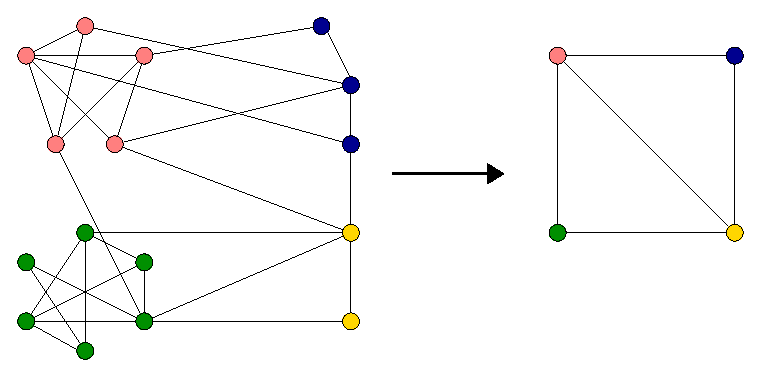
\includegraphics[width=0.50\linewidth]{img/mailing/graph-quotient}
	\vfill
	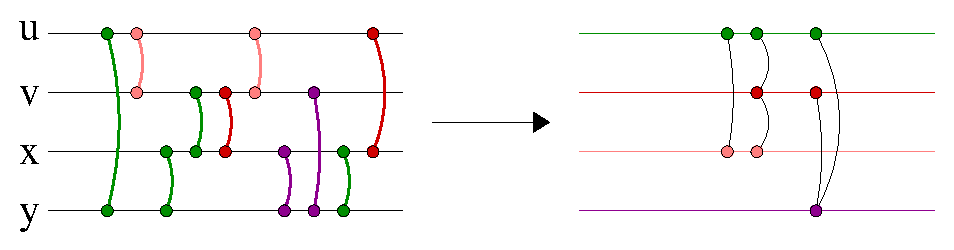
\includegraphics[width=0.75\linewidth]{img/mailing/stream-quotient}
	\caption{Haut: Exemple de graphe ayant une structure communautaire et son graphe quotient associé. Bas: Exemple d'un flot de lien avec une structure ainsi que son flot quotient associé.}
	\label{fig:graph-quotient}
%\label{fig:corel_inter}
\end{figure}

Nous étendons ici cette notion de graphe quotient aux flots de liens.
Nous définissons le flot quotient, $Q=(T_Q,V_Q,E_Q)$, induit par une partition $P=\{{P_i}\}_{1..k}$ en $k$ sous-flots de la manière suivante.
Chaque sous-flot $P_i$ est représenté par un n\oe ud dans $V_Q$.
Il existe un lien $(t,P_i,P_j)$ dans $E_Q$ si il existe $(t_1,u,v) \in P_i$, $(t_2,u,v') \in P_j$ et $(t_3,u,v'') \in P_i$ avec $t_1 \leq t_2 \leq t_3$.
En d'autre termes, il y a un lien dans $E_Q$ si un n\oe ud $u$ a un lien dans $P_j$ qui apparait entre deux autres de ses liens du groupe $P_i$.

Le flot quotient induit par les discussions dans le jeu de données contient 12281269 liens impliquant 68524 discussions différentes.
Comme notre jeu de données contient 116999 discussions, il y a donc 48475 discussions étant reliées à aucune autres et qui ne seront pas pris en compte par la suite.
Ce nombre de discussions non-reliées est élevé comparé à ce qui est obtenu dans un graphe. En effet dans un graphe, un n\oe uds non-relié corresponds à une communauté qui soit une composante connexe.
En ajoutant l'information temporelle, les discussions sont séparées par le temps dans flot.
C'est pourquoi un grand nombre de discussion ne sont pas reliées dans le flot quotient.
Ce phénomène est d'autant plus présent pour les petites discussions.

Il faut aussi noter qu'il y a environ 20 fois plus de liens dans le flot quotient que dans le flot initial.
Cela est normal car un lien dans le flot peut donner lieu à plusieurs liens dans le flot quotient.
Ce cas est visible sur la figure~\ref{fig:graph-quotient}. 
Le lien $(x,y)$ du groupe violet du flot à gauche donne lieu au lien $(\textcolor{plum}{violet}, \textcolor{red}{rouge})$ et au lien $(\textcolor{plum}{violet}, \textcolor{oliveGreen}{vert})$ dans le flot quotient à droite. 

\begin{figure}
\centering
	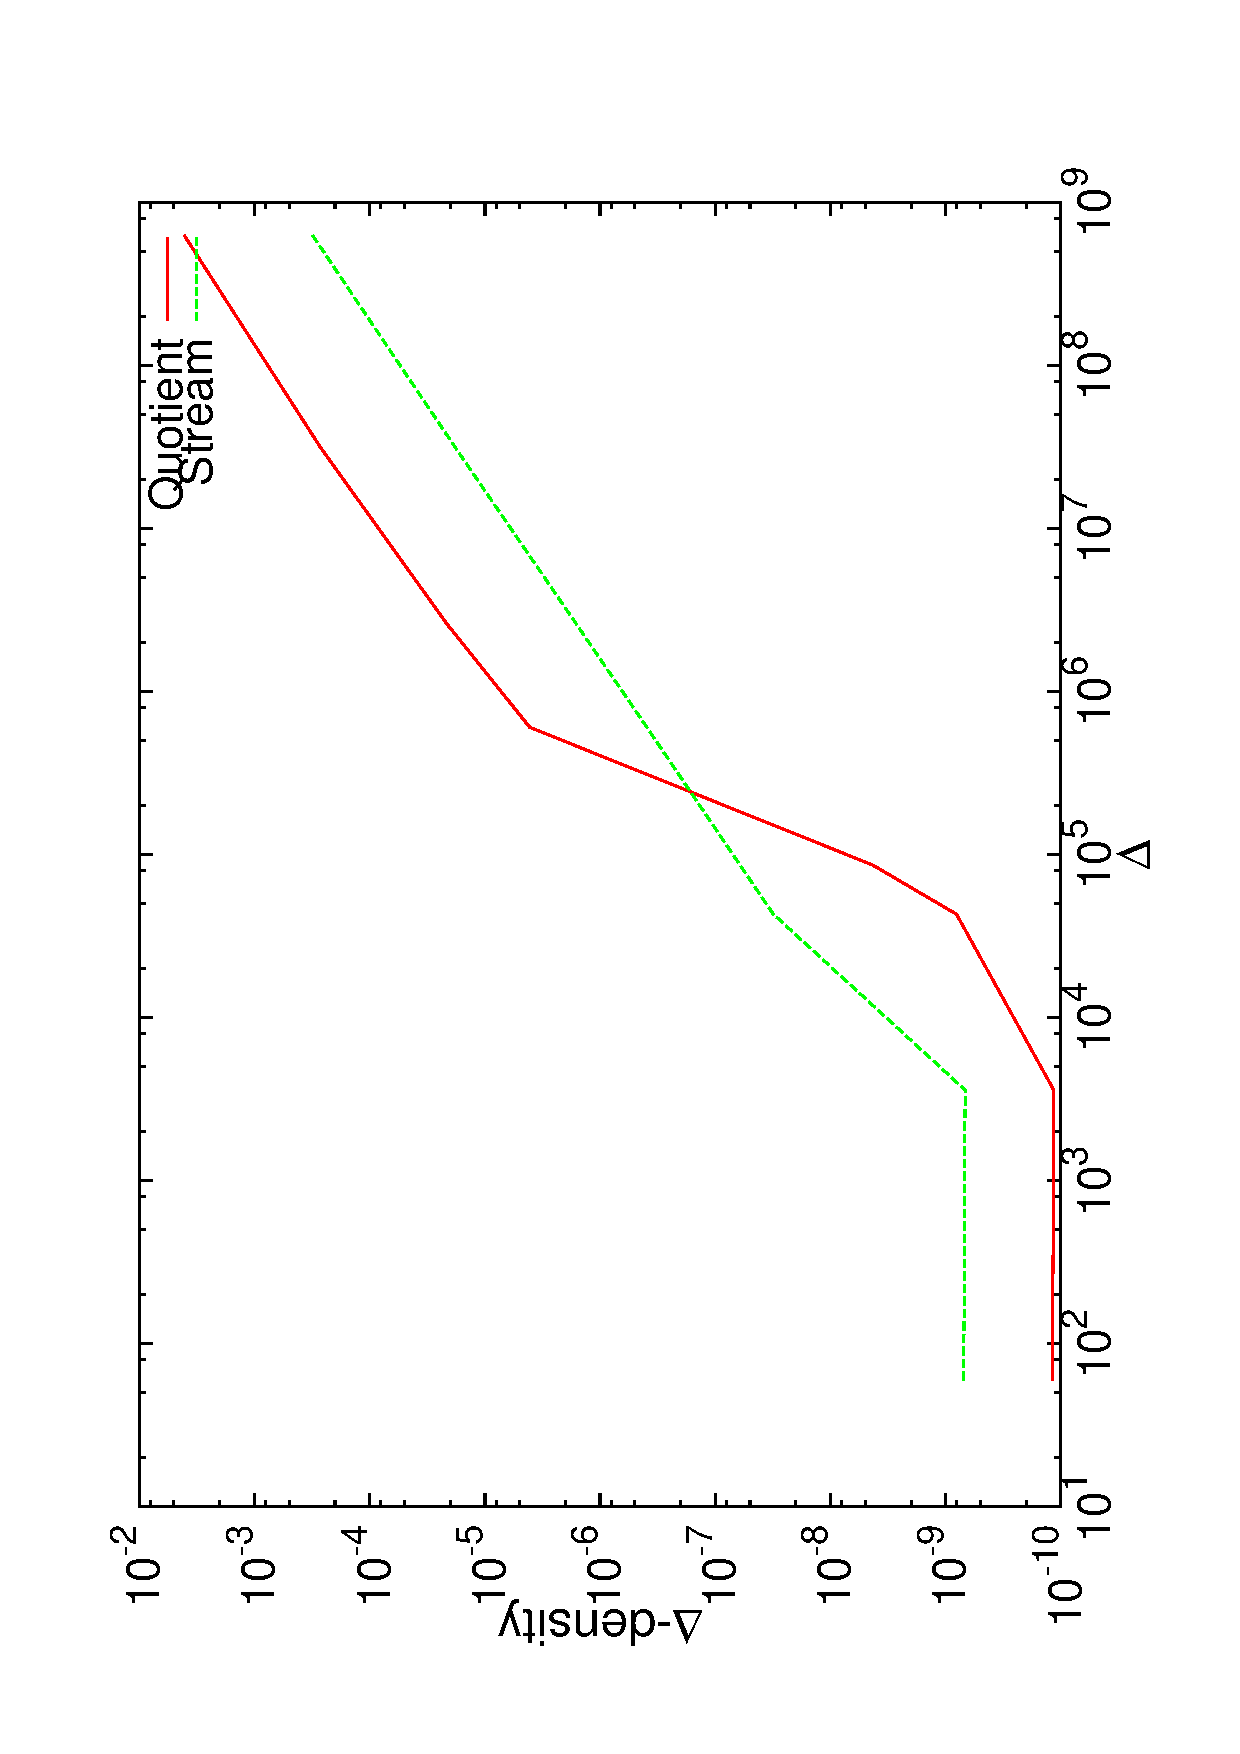
\includegraphics[angle=-90, width=0.71\linewidth]{img/mailing/quotient-density}
	\caption{$\Delta$-densité du flot de liens et du flot de liens quotien en fonction de $\Delta$ pour $\Delta=1mn, 1h, 12h, 1j, 7j, 30j, 1\ an$ et $20\ ans$.}
	\label{fig:quotient-stream-density}
\end{figure}

La figure~\ref{fig:quotient-stream-density} présente la $\Delta$-densité du flot de liens initial et du flot quotient pour différentes valeurs de $\Delta$.
Le flot quotient est plus $\Delta$-dense que le flot initial pour des valeurs de $\Delta$ importante.
Ce résultat est comparable a ce qui est obtenu dans un graphe.

\subsection{Conclusion}

Nous avons utilisé le modèle de flot de liens pour étudier une archive de courriels provenant du projet Debian.
Grâce au modèle de flot de liens, nous avons étudié des notions clefs pour mieux comprendre la répartition temporel et topologique des discussions.
Nous avons étudié la notion de $\Delta$-densité sur les discussions en elle même.
Puis, nous avons étudié les relations entre les discussions avec la $\Delta$-densité inter discussions, les projections en graphe de chevauchement temporel ou topologique et le flot quotient.

Cette étude repose en grande partie sur la notion de $\Delta$-densité qui nécessite un paramètre fixé arbitrairement.
Nous avons à chaque fois testé un ensemble de valeurs de $\Delta$ variant d'une seconde jusque parfois 20 ans et, lors de ces tests, aucune valeurs $\Delta$ caractéristique n'a pu être identifiée.
Il semble donc que la $\Delta$-densité soit relativement robuste vis-à-vis de $\Delta$ dans ce contexte.

Nous avons tout d'abord observé que les discussions forment une structure plus dense que le flot de liens.
De manière encore plus forte, nous avons constaté, grâce à la  $\Delta$-densité inter discussion, que les discussions sont plus dense en interne qu'en externe.
C'est une caractéristique importante des communautés que l'on trouve dans les graphes mais qui n'avait pas été observée dans un contexte temporel.
\`A partir de ces observations, nous avons également observé les relations entre les discussions.
Via le graphe de chevauchement temporel, nous avons validé le fait que différentes discussions ont lieu en même temps et que par conséquent une agrégation temporel entrainerait une perte d'information.
De même via le graphe de chevauchement topologique, on remarque que la structure est très recouvrante sur les n\oe uds, rendant ainsi l'utilisation de partitions statiques de n\oe uds difficilement envisageable pour décrire les discussions.


\inline{On a pas étudié de mesure spéciale graphe sur X ou Y.}
\inline{Faire évaluation des threads comme pertinent.}

\section{Détection de structures denses}

\`A partir du constat que les discussions forment une structure particulière, il est naturel d'essayer de les retrouver automatiquement. 
Pour y parvenir, il faut un moyen capable de trouver des sous-flots-denses dans le flots.
C'est à dire une méthode capturant des ensembles liens qui ont beaucoup qui soient proche temporellement et topologiquement.
Il serait tentant de directement d'optimiser la densité dans le flot mais ce n'est pas envisageable car un groupe constitué d'un unique lien a une densité de $1$.
Il faut donc trouver une autre méthode.
C'est pourquoi nous avons construit une projection du flot en un graphe statique afin d'y appliquer une méthode de détection de communautés.
Le problème est alors de réussir à créer une transformation de telle sorte que les informations temporelles et topologiques ne soient pas complètement détruites.

\subsection{Méthode de détection}

Dans la transformation que nous appliquons, nous créons un graphe non-orienté et non-pondéré $\mathcal{G} = (\mathcal{V},\mathcal{E})$.
Chaque lien du flot est représenté par un n\oe ud $\mathcal{V}$.
Deux liens $(b,e,u,v)$ et $(b',e',u',v')$ sont connectés dans le graphe s'ils partagent un n\oe ud, \emph{i.e.} $\{u,v\} \cap \{u',v'\} \neq \emptyset$, et si les intervalles s'intersectent, \emph{i.e.} $[b,e]\cap[b',e'] \neq \emptyset$, voir figure~\ref{fig:Transformation}.
Ainsi, un lien dans le graphe représente une connexion structurelle et temporelle entre deux liens du flot de liens.
Les groupes denses dans le graphe représentent donc des groupes de liens connectés temporellement et topologiquement dans le flot.

\begin{figure}
\centering
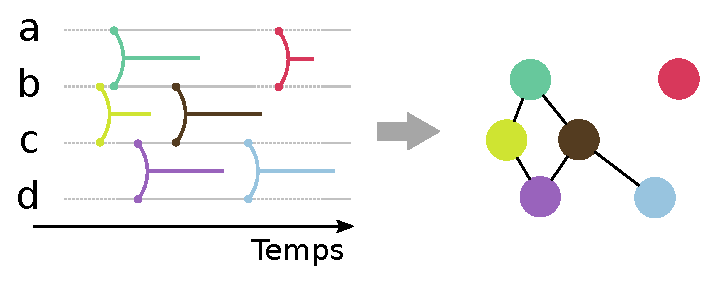
\includegraphics[width=0.6\linewidth]{img/mailing/Transformation.eps}
\caption{Transformation d'un flot de liens avec 4 n\oe uds (a-d) et 6 liens à gauche en un graphe à droite à 6 n\oe uds. La couleur d' un n\oe uds dans le graphe indique le lien du flot qu'il représente.}
\label{fig:Transformation}
\end{figure}%

Cette définition n'est valide que pour un flot de liens avec durée.
Or, les courriels échangés n'ont pas de durées.
Lors du calcul de la densité dans la section~\ref{delta_densite}, nous avions ajouté une durée arbitraire $\Delta$.
Ici, il n'est pas très pertinent d'appliquer la même logique.
En effet si on utilise un $\Delta$ faible, alors il n'y aura que très peu de liens dans $\mathcal{E}$ et les n\oe uds représentant les liens d'une discussions ne seront pas forcément connexes.
Il parait illusoire d'espérer retrouver les discussions dans $\mathcal{G}$ si elles ne sont même pas connexes.
C'est pourquoi nous adoptons une autre manière d'ajouter du temps.

Pour chaque message $m$, nous connaissons $p(m)$, le message auquel il réponds dans la discussion.
Nous définissons un autre flot, $\mathfrak{L}$, où les liens représentant les messages sont de la forme $(t(p(m)),t(m),a(m),a(p(m))$.
Ainsi, deux messages, $m_1$ et $m_2$, se succédant dans une discussion sont par définition reliés topologiquement car $a(m_1)= a(p(m_2))$.
Ces deux messages sont aussi reliés temporellement car  nous avons la relation suivante:
\begin{align*}
[t(p(m_1)),t(m_1)]\cap [\mathbf{t(p(m_2))},t(m_2)] &= \\
[t(p(m_1)),t(m_1)]\cap [\mathbf{t(m_1)},t(m_2)] &= [t(m_1)] \neq \emptyset.
\end{align*}
Par construction, une discussion est donc représentée dans $\mathcal{G}$ par un ensemble connexe de n\oe uds.


Un fois $\mathcal{G}$ construit, on peut appliquer un algorithme de détection de communautés.
Avec cette construction, $\mathcal{G}$  contient plus d'1 millions de liens pour les 116999 discussions présentes.
Sur ce graphe, nous avons appliqué l'algorithme de Louvain~\cite{Blondel2008a} qui optimise la modularité.
D'autres algorithmes peuvent également être appliqués s'ils cherchent un des groupes de n\oe uds disjoints et qu'ils passent à l'échelle.
Les groupes trouvés par Louvain sont des communautés dans $\mathcal{G}$.
Par conséquent, ils sont censé être densément connectés dans $\mathcal{G}$.
Comme un lien de $\mathcal{G}$ correspond à une connexion temporelle et topologique dans le flot, on peut espérer qu'ils correspondent à des groupes denses dans le flot.

\subsection{Comparaison des partitions}

Avant de comparer la structure des discussion, $D$, et la partition, $\mathfrak{D}$, trouvée par la méthode de Louvain sur $\mathcal{G}$, il est nécessaire de décrire cette dernière.
Sur la figure~\ref{fig:carac_mail_louvain}, les distributions cumulatives inverses des durées, du nombre n\oe uds et du nombre de liens sont présentés pour les groupes de $\mathfrak{D}$.
En pointillées, sont représentées les même données pour les discussions.
On remarque tout de suite que $\mathfrak{D}$ contient des groupes beaucoup plus gros et plus long, avec des groupes ayant jusque \com{X} liens et durant \com{X} secondes.
\begin{figure}[]
\centering

\caption{\com{Afaire}}
\label{fig:carac_mail_louvain}
\end{figure}

Ces deux structures sont donc très différentes mais cela pourrait être dû à l'algorithme de Louvain qui n'est pas adapté pour trouver des groupes denses.
C'est pourquoi, nous avons également la densité des groupes de $D$ et $\mathfrak{D}$ dans le flot $\mathfrak{L}$.
Le résultat est visible sur la figure~\ref{fig:dens_mail_louvain}.
Comme les liens de $\mathfrak{L}$ ont une durée, il est possible d'utiliser directement la densité au lieu de la $\Delta$-densité utilisée précédemment.
On remarque que les groupes de $\mathfrak{D}$, bien que plus gros, sont plus denses que les groupes de $D$.

\begin{figure}[]
\centering

\caption{\com{Afaire}}
\label{fig:dens_mail_louvain}
\end{figure}
\inline{Correlation taille/densité}

Si les groupes de $\mathfrak{D}$ sont plus denses, c'est peut être car ils regroupent plusieurs discussion de $D$ dans groupe.
Afin de mesurer cela, nous observons l'indice de Jaccard.

\begin{figure}[!h]
\centering
\hfill
\subfloat[niveau 0]{
%\includegraphics[width=0.3\linewidth]{}
}\hfill
\subfloat[ niveau 1]{
%\includegraphics[width=0.3\linewidth]{}
}\hfill
\subfloat[niveau 2]{
%\includegraphics[width=0.3\linewidth]{}
}
\hfill
\caption{\com{[Afire]}.}
\label{fig:rec_inclusion}
\end{figure}
